\documentclass{article}
\usepackage[utf8]{inputenc}
\usepackage{graphicx}
\usepackage{hyperref}
\usepackage{subcaption}
%\usepackage{amsmath}
%\usepackage{multirow}
%\usepackage{multicol}
\title{DPhil: Thesis}
\author{Shaan Desai }


\begin{document}

% Title page is created here
\maketitle


%%%%% DEDICATION -- If you'd like one, un-comment the following.
%\begin{dedication}
%This thesis is dedicated to\\
%someone\\
%for some special reason\\
%\end{dedication}

\tableofcontents


\section{Literature Review (WIP)}

\subsection{Artificial Intelligence}

- Humans have long tried to understand how the mind works
- from a biological perspective it is clear that connectomics paves a pathway to understanding how we think
- With the advent of computers and 'large' processing power, many researchers began to ask whether the human mind can be replicated using a computer.
- Early work by walter and warren was the first to point out a means to build neural network logic.
- Followed by Hebbian
- Then an AI winter
- Geof Hinton backprop
- slew of advents in neural processing, convnets, rnns, graphs, tensor nets, deep RL, 
- all seeking to solve more tasks/increase generalizability.
- to date, there has been no general purpose solution (AGI) for a vast array of tasks e.g. a human can learn to create art, sit math exams, play sports, yet a robot so far can only do one of these tasks well.
- Numerous limitations in terms of processing power and memory access still exist

- Despite these limitations, neural networks have brought about significant advancements to society in robotics, self driving cars, cancer detection.

- In what follows, we outline some of the major advances, those which have been fundamental pillars to research conducted during this phd. We follow no particular order.

\subsection{Inductive Biases}

An inductive bias in machine learning is prior information used to guide model building. In simple linear regression, for example, we assume the distribution of the noise in our data follows a Gaussian. This is a natural inductive bias because prior to seeing any data, we have assumed our noise model follows this form. In neural networks, architectures with variable depth, form and activations for example, serve as inductive biases. In essence, we encode initial assumptions about the complexity of data via inductive biases. 

A feedforward deep neural network naturally encodes 'nonlinearity' as a prior and arguably makes the least assumptions about the underlying data. Convolutional Neural Networks assume spatial representations can be captured. Recurrent Neural Networks assume temporal data as inputs. 

In what follows, we highlight some of the recent advances in inductive biases, particularly as they relate to solving problems in physics.

\subsection{Graph Neural Networks}

Graph Neural Networks are neural networks which use graphs as inputs. As such, they can be used to understand and learn the relationships which exist between the nodes of a graph. More formally, a graph is a tuple (Vertices,Edges,Globals). These are attributes of the graph where the nodes contain information, edges contain relationship weights and globals consist of macro variables general to all graphs. 

interaction-physics based problems naturally benefit from graphs. We see that HOGNs and OGNs achieve great results in rolling out trajectories of N body systems. 

Although they account for a new set of relational inductive biases, graphs still involve complex message passing schemes that involve significant fine-tuning. In addition, they assume data streams are already structured. However, graphs have shown significant promise in physics e.g. in explaining the phase transition of glassy materials. Their use in physics opens up a tried-and-tested pathway to solve more complex problems particularly in accounting for material interactions. 

They're even shown to model complex fluid like systems from visual data. 

Most systems to date have looked at graphs for classical physics but literature from 2004 suggests graphs, inherent in their relational structure, can also capture Ising-like hamiltonian structure.


\subsection{Symplectic Biases}

Symplecticity refers to the concept of volume-preservation. Riemannian**
Core to our beliefs in physical systems is the notion of energy conservation, indirectly accounted for by symplecticity.

\subsection{Integrative Biases}
- ODEnet
- new paper by tegmark

\subsection{Physics priors}


Broadly, the intersection of physics and AI falls into one of two domains, physics for AI or AI for physics. The former uses techniques from physics to develop and improve learning algorithms in general, for example xx. The latter uses existing learning approaches (with adaptations) to predict physics, for example ML for materials. In this review, we focus our attention on the latter.

Physicists have long been interested in using learning tools to predict physics based systems. Some of these include predicting magnetic properties of 2-D materials, predicting the time evolution of N-body systems and even using AI to understand phase transitions. However, numerous challenges still remain in terms of data-efficient learning, reducing computational cost, improving predictive accuracy and learning better representations of the underlying physical process. Researchers have identified methods to address these challenges, but arguably the most promising hinges on physics-informed priors embedded in learning. It has been shown that models enriched with physically-informed priors i.e. models which consist of some knowledge about the physical system apriori, significantly outperform traditional methods in terms of data-efficiency and predictive accuracy. This has sparked a sharp interest in building both task-specific and general physics priors to improve learning. In this section, we summarize some of the core developments over time in physics informed inductive biases. 

\subsubsection{gradient learning}


The notion of embedding physically-informed inductive biases in neural networks can be found in numerous early work aimed at modelling materials \cite{witkoskie_neural_2005, pukrittayakamee_simultaneous_2009, smith_ani-1_2017, rupp_fast_2012, yao_tensormol-01_2018}. For example, early efforts by Witkoskie and Doren \cite{witkoskie_neural_2005} demonstrate that in contrast to directly learning a potential energy surface, the inclusion of gradient learning can drive a network to accurately model the forces. This addition means that we supplement the learning process with additional information and hence improve the learnt potential surface. 




\subsubsection{Hamiltonian Neural Networks}

ing neural networks to accurately learn classical dynamics from data  problems has been Hamiltonian Neural Networks \cite{greydanus_hamiltonian_2019}. In  demonstrated that dynamic predictions through time can be improved using Hamiltonian Neural Networks (HNNs) which endow models with a Hamiltonian constraint. The Hamiltonian is an important representation of a dynamical system because it is one of two approaches that generalizes classical mechanics. The Hamiltonian $\mathcal{H}$ is a scalar function of position $\mathbf{q} = (q_1,q_2,....,q_M)$ and momentum $\mathbf{p} = (p_1,p_2,....,p_M)$. In representing physical systems with a Hamiltonian, one can simply extract the time derivatives of the inputs by differentiating the Hamiltonian with respect to its inputs (see Eqn. \ref{eqn.hamiltonian}.)
\begin{equation}
\frac{\mathrm{d}\mathbf{q}}{\mathrm{d}t} = \frac{\partial \mathcal{H}}{\partial \mathbf{p}}, ~~~
\frac{\mathrm{d}\mathbf{p}}{\mathrm{d}t} = -\frac{\partial \mathcal{H}}{\partial \mathbf{q}}
\label{eqn.hamiltonian}
\end{equation}
As a consequence, it is noted in \cite{greydanus_hamiltonian_2019} that by accurately learning a Hamiltonian, the system's dynamics can be naturally extracted through backpropagation. This information allows us to build two 1st-order differential equations which can be used to update the state space, $(\mathbf{q},\mathbf{p})$. Equation \ref{eqn.action_int} shows this integral, in which we define the symplectic gradient $\mathbf{S}  = \left [ \frac{\partial \mathcal{H}}{\partial \mathbf{p}},-\frac{\partial \mathcal{H}}{\partial \mathbf{q}} \right ] $:
\begin{equation}
(\mathbf{q},\mathbf{p})_{t+1} = (\mathbf{q},\mathbf{p})_t + \int_t^{t+1} \mathbf{S}(\mathbf{q},\mathbf{p}) \mathrm{d}t
\label{eqn.action_int}
\end{equation}
%However, this is not the only benefit in learning a Hamiltonian. Another key attribute of the Hamiltonian is that the vector field $\mathbf{S}$ is a symplectic gradient meaning $\mathcal{H}$ remains constant as long as state vectors are integrated along $\mathbf{S}$. This result links the Hamiltonian with the total energy of the system $\mathcal{H}(\mathbf{q},\mathbf{p}) = E_{tot}$. 
It can be shown that the Hamiltonian in many systems also represents the total energy of the system. Therefore, the Hamiltonian is a powerful inductive bias that can be utilised to evolve a physical state while maintaining energy conservation.



\section{Notes}

A section to document some of my learnings over time.

\subsection{GANs for Physics (Oct '19 - Jan '20)}

\subsubsection*{Preliminary Ideas}

Can generative networks capture the laws of physics?

\begin{enumerate}
\item Generative networks are able to learn complex mappings from data to latent spaces
\item Often, these latent spaces are able to perfectly generate the original data which might indicate that the fundamental laws of physics are being captured by the network
\item This leads us to the question - can we use a generative network to learn dynamics of a particle e.g. in the 2 body problem, and observe whether the generator learns the underlying equations of motion.
\end{enumerate}
Key point: if i can generate the data, I must understand something about the laws of physics.

Inspired by greydanus, we wondered if a GAN-like approach can be taken to model and understand the phase-space.

\subsubsection*{GAN Theory}

What is a Generative Adversarial Network?

Intuition is that there is an art forger (G) and art critique (D) who are tasked with making and evaluating art respectively. 

\begin{enumerate}
\item $\hat{x} = G(z) $ where z is noise and $\hat{x}$ has to match the distribution of $p(x)$.

\item $D(x)$ is a mapping into a probability. Discriminates between real and fake art.
\end{enumerate}

They are adversaries, as such, they have different cost functions to optimize. This induces Nash equilibria:

It is a game between 2 players in which the equlibria is a local minima for each loss. This means the generator draws samples perfectly from $p(x)$ and the discriminator cannot discriminate so predicts 1/2 for all samples.

The discriminator loss follows that of a log bernoulli distribution or the cross entropy loss function.

$$ H(p,q) = -\sum_i p_i \log q_i$$

For binary classification we get:

$$ H((x_1,y_1),D) = -y_1 \log D(x_1) - (1-y_1) \log (1-D(x_1)) $$

If we sum over each value in the dataset, we then obtain:

$$ H((x_i,y_i)_i^N,D) = -\sum_{i=1}^N y_i \log D(x_i) - (1-y_i) \log (1-D(x_i)) $$


Now ideally, we like to take this and make some changes.

\begin{enumerate}
\item we want data to be split evenly, so if the total dataset size is N. We set N/2 of the samples to be class 1 and N/2 to be class 0. This automatically reduces the above y variables to 1/2's. 
\item The x values come from 2 sources. The legitimate source and the sampled source. We want this to be probabalistic so sums become expectations.
\end{enumerate}

%$$ H = -\frac{1}{2} \mathbb{E}_{x \sim p_{data}} [log D(x)] - \frac{1}{2} \mathbb{E}_{\hat{x}  \sim p_{model}} [log(1-D(\hat{x}))] $$ 
%
%
%$$ H = -\frac{1}{2} \mathbb{E}_{x \sim p_{data}} [log D(x)] - \frac{1}{2} \mathbb{E}_{z} [log(1-D(G(z)))] $$ 

The discriminator needs to minimze the above loss. It is the same as the cross-ent loss for a NN doing binary classification with sigmoid output.

If we optimize this loss holding G constant, we get:

$$ D(x) = \frac{p_{data}}{p_{model} + p_{data}} $$

This is nash equilbrium.

Zero-sum game means any loss is conserved between entities. 

The zero sum game solution is minimax where we want to minimize the maximum loss. The discriminator wants a higher payoff so tries to maximize while the generator wants a lower loss so minimizes. To optimize this, an interative approach is used.


The sources used to understand these concepts come from \href{https://seas.ucla.edu/~kao/nndl/lectures/gans.pdf}{ucla tutorial} and \href{https://danieltakeshi.github.io/2017/03/05/understanding-generative-adversarial-networks/}{Takeshi github link}.



\subsubsection*{Training GANs}

To start we  train a GAN using MNIST (Adam optimizers and saw convergence). We attempted GAN with pendulum motion and saw multiple convergence issues. We notice some challenges with training GANs - generator usually diverges while discriminator rapidly converges. Many tips online i.e. make target values 0.9 instead of 1 to reduce certainty.Using ‘hacks’ only can see marginal improvement. Larger issue of GANs being unstable.

Furthermore, do we actually want to use GANs for the application? Seems that the only way to constrain the noise input is to encode it which essentially gives us an autoencoder.

VIN network is a good idea though we have no code base/architecture used.

Attempted to use AE-GAN to encode physics and also build a discriminator: challenge at the moment is discriminator loss is increasing (rare) and predicted output images look nothing like the ground truth. 

Some ideas:

\begin{enumerate}

\item Changed optimizers
\item Changed network architecture
\item Removed discriminator and still noticed issues
\item Even when architecture is consistent with HNN
\item Perhaps the only difference is torch.randperm and torch shuffle
They use shuffling of data with replacement and don’t use epochs but steps
\item Takens theorem \href{https://en.wikipedia.org/wiki/Takens%27s_theorem}{here}
\end{enumerate}


Not necessarily evident what the benefits are of having the AE-GAN from the simple autoencoder network/ perhaps better images but this might not improve the latent space we learn.

An alternative approach is to sample the latent space in a way which is consistent with the laws of physics (i.e. sample p and q) sequentially, as we sample the ground truth images - then we can see how p,q can ‘map’ into a 2D image (might be potential to learn from the hidden layers) but this is fully supervised and we are not learning anything immediately useful.

Some experimental results
\begin{figure}[h!]
\centering
\begin{subfigure}{0.7\textwidth}
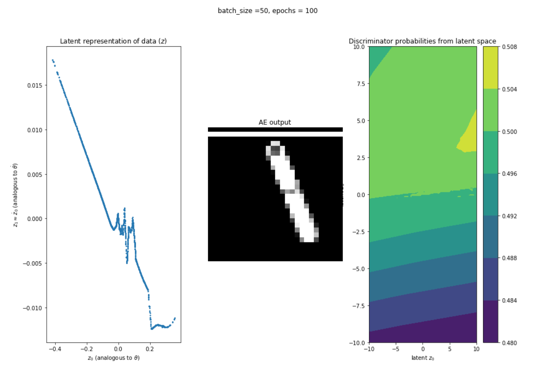
\includegraphics[width=\textwidth]{figures/gan_phase_1stack.png}
\end{subfigure}
\begin{subfigure}{0.7\textwidth}
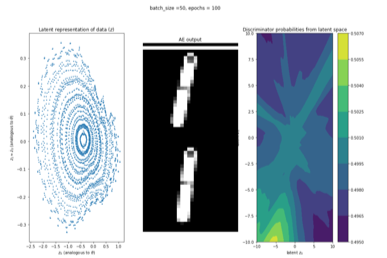
\includegraphics[width=\textwidth]{figures/gan_phase_2stack.png}
\end{subfigure}
\begin{subfigure}{0.7\textwidth}
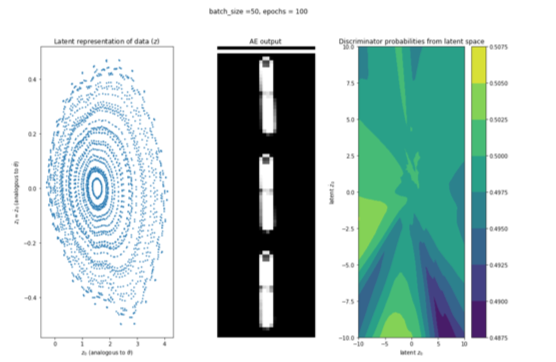
\includegraphics[width=\textwidth]{figures/gan_phase_3stack.png}
\end{subfigure}
\end{figure}

We carried out an extensive study between batch size and epoch. However, we find no consistency in the generated phase space.

\subsubsection*{key takeaways}

Preliminary results show that GANs are difficult to work with (this could be an interesting topic to cover on its own). I believe gradient clipping is one way to solve this issue. 
More importantly, Variational Integrator Networks proves that the learnt phase space from an AE will not, in general, represent the true phase space. In order to do this, one needs to encode the Lie group dynamics.
Constrained GANs have already been looked at for generating consistent results.

We still have yet to establish why a potential Lie group constrained GAN can help the world. i.e. why is it useful to be able to generate random samples of a pendulum swinging?


\subsection{VIGN}

Need to fill this section out in detail.


\subsection{Lagrangian Dynamics (WIP)}
The Euler-Lagrange formulation equates to:

$$ \frac{\partial}{\partial t} (\frac{\partial L}{\partial \dot{q}}) = \frac{\partial L}{\partial q} $$

where:
$$ L = T - U $$

In the example of a pendulum:

$$ T = 1/2 mv^2 = 1/2 m (l\dot{\theta})^2 = 1/2 m l^2 \dot{\theta}^2 $$

$$ U = mgh = mgl(1- \cos \theta) $$

$$ L = 1/2 m l^2 \dot{\theta}^2 - mgl(1-\cos\theta) $$

Placing the above into the euler-lagrange form gives us:

LHS:

$$ \frac{\partial L}{\partial \dot{q}} = ml^2 \dot{\theta}$$

$$ \frac{\partial}{\partial t} (\frac{\partial L}{\partial \dot{q}}) = ml^2 \ddot{\theta} $$

RHS:

$$ \frac{\partial L}{\partial q} = -mgl\sin\theta$$

Therefore:

$$ \ddot{\theta} = \frac{g}{l} \sin \theta $$


Now, to transition to the Hamiltonian version:

We can write the hamiltonian as the sum of the energies:

$$ H = T + U $$

$$ H = p^2/2m + U $$

$$ H = -L + 2K $$

$$ H = -L + mv^2$$

$$ H = -L + p^2/m = -L + p* (m\dot{q})/m = -L + p\dot{q}$$

$$ p = \frac{\partial L}{\partial \dot{q}} $$


\section{Running Ideas}

\subsection{VIGN extension}

- non conserved energy domain
is there a link between the port-hamiltonian view and lagrangians with generalized force
for a damped system we have:

$$ \frac{d}{dt} \frac{\partial \mathcal{L}}{\partial \dot{q}} - \frac{\partial \mathcal{L}}{\partial q} = \mathbf{F}^{ext} \frac{\partial \mathbf{r}}{\partial q}$$

see \href{http://www.physics.hmc.edu/~saeta/courses/p111/uploads/Y2013/lec131023-DSHO.pdf}{here} for details on how this equation was built. 

- distributional assumptions for practical purposes

Assume $ H = E_c $ for a trajectory of an initial condition, then:

$$ H = K + U $$

$$U = H - K $$

$$ L = K - U $$

$$ L = 2K -H $$

Now, for L to be constant, K needs to be constant. In most cases, $ K = p^2/2m $. For this to be constant p should be constant. For p to be constant, $\dot{p} = 0$. This would imply, for most settings, that:

$$ \frac{dp}{dt} = \frac{dU}{dq} = 0 $$

This means that U is zero, which is not true.

We have proven that as long as energy is conserved in a system exhibiting $K = p^2/2m$ the Lagrangian will never be constant unless the system has 0 potential. 

As such, the Lagrangian depends on the distribution of the kinetic energy/potential energy. In the large N limit, these distributions tend toward a Gaussian.

Is it beneficial to have a target variable distributed more broadly like a gaussian vs a delta?


\subsection{Covid}


SEIR model is differentiable and has some hamiltonian/energy conserving property. how might we build a neural network on this?

We start out using SEIR to model china and it works well.

We have issues modeling beijing which is seeing a second spike, we could reshape R naught (t) as an exponential sine function.
$$ R_0(t) = Ae^{-(t-t_0)}|sin(B(t-t_0))| $$

This is too specific. How can we encode the SEIR model into a graph neural network. Note, graph networks and graph neural networks are different frameworks encompassing the same core operations. In graph networks, however, the intermediate functional representations (hidden layers) are computed first, before an aggregation scheme is used. In graph neural networks, e.g. GCN, the operations involve computing a hidden layer first using neighbouring nodes, before feeding these hidden layers into the graph neural network.

This reversal means one needs to be careful in how they define graph neural network architectures between DGL and deepmind graph nets library.

We use graph convolutions to train on simulated data, we find hypersensitivity to initial conditions. More importantly, because of the time dependent nature of the system we are unsure of how many lag-variables are necessary to evolve the system.

\subsection{Inductive  biases for RL}

MDPs with policies which are deterministic or stochastic. Model free which involves sampling at random. Model based which involves sampling the learnt environment.






\end{document}
